%%%%%%%%%%%%%%%%%%%%%%%%%%%%%%%%%%%%%%%%%%%%%%%%%%%%%%%%%%%%%%%%%%%%%%%%%%%%%%%%
%%% Problem statement
%%%%%%%%%%%%%%%%%%%%%%%%%%%%%%%%%%%%%%%%%%%%%%%%%%%%%%%%%%%%%%%%%%%%%%%%%%%%%%%%

\clearpage
\section{Problem Statement}
\label{sec:problem}

%% intro
In this section I will describe the store backend system examined in this thesis (later: \textit{system}) 
and elaborate on the problems that I was solving in this project (later: \textit{project}). 
I will also describe the users of the project and what the needs for
each of them were, as discovered by the requirements engineering work I did.

%% description of the store
%% ingestion system
%% workflows, processors, parallelism
%% description of the terms used

\subsection{The store systems}

The system being investigated in this thesis was the Microsoft Windows store.
The store sells digital \emph{products} such as games and applications.
Each product belongs to a \emph{publisher} such as an independent developer or a game company.
A product is \emph{submitted} by a publisher as a digital application package.
Before it is \emph{published} to the store catalog, it needs to be \emph{ingested},
which means the package is verified and processed through multiple steps.
After the package has been ingested and the necessary information has been collected,
it can be published, which also involves a pipeline of steps.
These steps together form an ingestion-publishing \emph{workflow} that consists of multiple \emph{activities} (steps).
Completion of each of these activities is logged as an \emph{event}.
The list of events for a single submission forms a \emph{trace}.
These terms will be used throughout this thesis so they shall be formally defined as follows:

% describe: workflow, trace (submission), product (bigid), publisher, event

\begin{description}[style=nextline]
\item[Product] 
Single digital application package being processed in the system. 

\item[Publisher] 
Independent developer or a company submitting a product that they own into the store.

\item[Activity] 
Single atomic step of the workflow, where some part of the product is processed. 

\item[Processor] 
Part of the distributed system executing a specific activity.

\item[Workflow]
Abstract description of the whole pipeline consisting of a number of sequential and parallel activities. It contains the whole set of activities and their dependencies.

\item[Submission] 
Single execution of the workflow for a single product. Equates to a single \emph{case} in the process discovery model.

\item[Event] 
Log entry documenting the time when a specific execution of an activity has finished or changed status. 

\item[Trace] 
Set of events describing a current or past submission. 
A trace is tied to a specific product from a specific publisher and has information about all the activities and their execution times. 

\item[System] 
The distributed store backend system as a whole, with all the processors and other parts involved.

\item[Project] 
The new part of the system implemented in this thesis.

\label{desc:termdefinitions}
\end{description}


%% logging
The workflows are processed in the distributed system as a pipeline of steps. 
Multiple concurrent submissions are in progress at any moment of time.
Furthermore, many steps of the workflow are independent of each other.
Thus, a single submission can have multiple steps in progress at the same time.
However, to continue the workflow all the parallel steps need to complete.
An ``aggregator'' step waits for the parallel steps to finish and only then proceeds to the next step. 
Figure \ref{fig:workflowexample} illustrates this.
The different steps of the workflow have different lengths that depend on, among others,
the processing needed, the characteristics of the package, and the current workload of the system.
Because of these uncertainties, traces from two different submissions may differ from each other.
The order, which the parallel finish, is unknown, as described in section \ref{sec:eventtheory}.

\begin{figure}[htb]
\centering 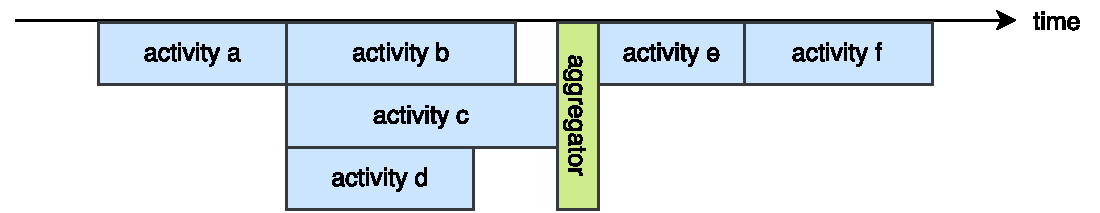
\includegraphics[width=0.9\linewidth]{gfx/figures/workflow.pdf}
\caption{A workflow with sequential, parallel, and aggregator steps}
\label{fig:workflowexample}
\end{figure}

When each step completes, an event is generated.
These events are collected from the different processors into a single database.
Each step is associated with a timestamp and all the available metadata.
The system works by a ``best effort'' delivery. 
This means the delivery of the events to the database can fail and thus be delayed.
Furthermore, the distributed system involves multiple machines in multiple locations. 
This results in variance of seconds to minutes in the clocks of the systems.
The clock variance is directly seen as noise in the timestamps of the events.

Because of the described parallelism and the uncertainties mentioned, the overall state of the system is difficult to describe at any given time.
Looking at the raw log data is also challenging because of the volume.
At the time of writing, the system produced on average 15~000 events per hour with peak times averaging in the 30~000 range.
Event filtering and visualization is necessary to find the relevant data from the noise.

\subsection{Requirements engineering}

%% description of users
% engineers, developers, working on ingestion
% first party and third party publisher release managers
% managers, PMs
In the beginning of my work the project requirements were not clear.
To understand the needs of the users, I conducted requirements engineering work.
In my research I discovered five user groups relevant to the project:

\begin{description}
\item[Developers] are the Microsoft software engineers working on the ingestion and publishing system.
\item[Managers] are the Microsoft developer leads and program managers who coordinate the developers' time and what they are working on.
\item[Publishers] are the independent creators, companies, and other third parties submitting the product packages to the store.
\item[Release managers] are Microsoft employees who have been assigned to be a contact for the largest publishing companies who develop the high-profile ``triple-A'' games and applications. 
\item[Manual reviewers] are the people working for Microsoft that do the manual steps of the product validation when necessary. This includes, for example, checking a submission for fraud or inappropriate graphics or language.
\end{description}

The needs for each user group are covered in table \ref{tab:userneeds}.
I used the ``user story'' format for documenting the needs \cite{cohn2004user}.

%% description that user needs were not fully known so they need engineering
The project was done in two cycles, with requirements engineering work done in the beginning of both cycles. See section \ref{sec:timeline} for the project timeline. 
The user needs found at the start of the second section were related mostly on the presentation and the user interface, so they did not affect the main structure of the project significantly.

%% description of initial user needs
% which?

\begin{table}[htb]
\begin{center}
\begin{tabularx}{\linewidth}{| X |}
\hline

\textbf{As a developer I want...} \newline
- to see the current status of a submission so that I can investigate issues with a single submission or product.\newline
- to see the shape of the store workflows so that I can find issues in the dependencies.\newline
- to see statistics about the activities so that I can write reports to my superiors.\newline
- to be able to customize what I see so that I can have exactly the information I care about.\newline
- to be notified of any delays in the workflow so that I can investigate issues faster.\newline
- to be notified about big issues distinctively so that I can prioritize my work.
\\
\hline

\textbf{As a manager I want...} \newline
- to have statistics of the workflows so that I can report the system performance and improvements over time to my superiors.
\\
\hline

\textbf{As a publisher I want...} \newline
- to be able to know estimated times for submission completion so that I can schedule my work day.\newline
- to be able to inquire about the status of my submissions so that I can escalate any issues that arise
\\
\hline

\textbf{As a release manager I want...} \newline
- to see the detailed status of a single product or submission so that I track it and report any issues to my superiors. \newline
- to see the big picture status for all submissions related to a single product or publisher quickly so that I can save time. \newline
- to be notified about completion of crucial steps of the workflow or any issues so that I can schedule and prioritize my work. \newline
- to be able to customize what I see so that I do not see information about products that I do not own.
\\
\hline

\textbf{As a manual reviewer I want...} \newline
- to be notified in advance when a product is heading towards a manual review so that I can schedule my work day.
\\
\hline

\end{tabularx}
\end{center}
\caption{Initial user needs found in January}
\label{tab:userneeds}
\end{table}

%% business requirements
%% need to integrate with an existing system
%% confidentiality, integrity
%% working with partners

The project also involved business requirements from Microsoft. 
The major two requirements were integration with existing systems and following confidentiality requirements.
The project was required to integrate with the existing store backend systems. 
The event collection and storing was already handled by a system called \textbf{Jury}, which is an interface to browse the products in the store and see diagnostics information from the log database.
The existing system stores the events in a database and allows the used to query the events with a SQL-like query language. 
The results were shown as a list of rows with the matching events and timestamps (see figure \ref{fig:plaineventlog}). 
The project was to integrate with this querying system to load the events from the database.
The events and the product metadata in the system contained confidential information. 
Mainly there were two terms used to classify confidential data: \textit{Medium Business Intelligence} (MBI) and \textit{Personally Identifiable Information} (PII). 
In practice, it meant that any MBI-classified information related to a product should only be shown to the publisher or the partner who owns the product.
For example, the product events should only be available to the publisher who owns the product.
However, the developers working at Microsoft should be able to see all MBI-classified information.
Any PII-classified information should be considered private and should not be visible through the interface developed in this thesis. 

%% challenges
%%  user needs not fully understood
%%  unknown parallelism
%%  unsupervised learning and adaptation
%%  both real time and statistical data are needed

There were several challenges discovered in the beginning of the project.
The system implemented in the project should be unsupervised.
This means that the system should use past data to build an understanding of the workflow without the need for a user such as an engineer to supply any knowledge beforehand.
The system should adapt to any changes in the workflow automatically.
The distributed workflows contain unknown parallelism that must be detected automatically.
Furthermore, the distributed system contains noise in the timestamps which further complicate the parallelism detection.

In addition, the system should be able to provide two different kinds of information. 
The workflow models and statistics should be built based on a long term aggregate discovered from several days worth of data,
while the system should also show the real time data for the current ongoing submissions.
These two sides of information should both be utilized in the visualization.
Lastly, requirements engineering was necessary to discover the user needs. 
This is why an iterative process was set up. 
Section \ref{sec:timeline} contains a detailed description of this process.

%% needs discovered at meetings?

%% conclusion, key goals
To recap, the key goals for the solution developed in this thesis are the ability to dynamically adapt to changes in the workflow,
the ability for the user to customize the information they need, and decoupling the solution from the specific workflow steps of the store. 
The project needs to use \emph{unsupervised learning} to build workflow models, show \emph{real-time event data} to the user based on the model, 
and use the models and the real-time data to show predictions of future events.
